\documentclass[a4paper,12pt]{article}
\usepackage[utf8x]{inputenc} %fac
%\usepackage[utf8]{inputenc} %fac

%\usepackage[square,sort,comma]{natbib}
%\usepackage{chapterbib}

\usepackage[francais]{babel} %FR
\usepackage[T1]{fontenc}
\usepackage{fancyhdr}

\usepackage[pdftex]{graphicx} % img
%\usepackage{wrapfig} %fac
\usepackage{float}

%\usepackage{algpseudocode} %fac
\usepackage[hidelinks]{hyperref} %fac

\usepackage[top=3.5cm, bottom=3.5cm, left=3cm, right=3cm]{geometry} %Réduire les marges

% \usepackage{showkeys}
% \usepackage{showlabels}
\usepackage{nameref}

% Style Page
\pagestyle{fancy} % entêtes

\setlength{\headheight}{15pt}
\lhead{ \leftmark }
\rhead{ %\rightmark 
}

\sloppy % ne pas faire déborder les lignes dans la marge

%\setcounter{tocdepth}{1} %hideallsubsections

\begin{document}
  \begin{titlepage}
   \def\titletype{Manuel du programmeur}
   %%%%%%%%%%%%%%%%%%%%%%%%%%%%%%%%%%%%%%%%%
% University Assignment Title Page
% LaTeX Template
%
% This template has been downloaded from:
% http://www.latextemplates.com
%
% Original author:
% WikiBooks (http://en.wikibooks.org/wiki/LaTeX/Title_Creation)
%
% Instructions for using this template:
% This title page is presently capable of being compiled as is. This is not
% useful for including it in another document. To do this, you have two options:
%
% 1) Copy/paste everything between \begin{document} and \end{document}
% starting at \begin{titlepage} and paste this into another LaTeX file where you
% want your title page.
% OR
% 2) Remove everything outside the \begin{titlepage} and \end{titlepage} and
% move this file to the same directory as the LaTeX file you wish to add it to.
% Then add \input{./title_page_1.tex} to your LaTeX file where you want your
% title page.
%
%%%%%%%%%%%%%%%%%%%%%%%%%%%%%%%%%%%%%%%%%

%----------------------------------------------------------------------------------------
%       PACKAGES AND OTHER DOCUMENT CONFIGURATIONS
%----------------------------------------------------------------------------------------

\begin{titlepage}

\newcommand{\HRule}{\rule{\linewidth}{0.5mm}} % Defines a new command for the horizontal lines, change thickness here

\center % Center everything on the page

%----------------------------------------------------------------------------------------
%       HEADING SECTIONS
%----------------------------------------------------------------------------------------

\textsc{\LARGE Pierre and Marie Curie University}\\[1.5cm] % Name of your university/college
\textsc{\Large \titletype}\\[0.5cm] % Major heading such as course name
%\textsc{\large PIAD de Master1 d’Informatique en Intelligence Artificielle et Décision}\\[0.5cm] % Minor heading such as course title

%----------------------------------------------------------------------------------------
%       TITLE SECTION
%----------------------------------------------------------------------------------------

\HRule \\[0.4cm]
{ \huge \bfseries \majortitle}\\[0.4cm] % Title of your document
\HRule \\[1.5cm]


%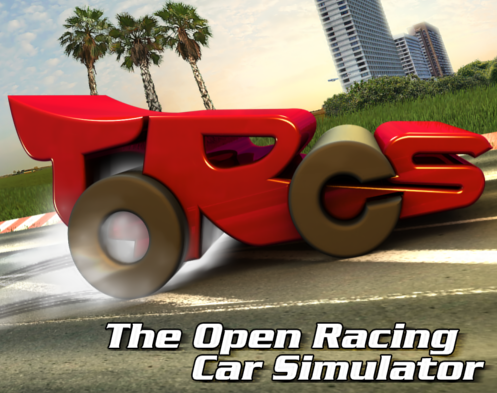
\includegraphics[height=60mm]{images/torcs.png}\\[1cm]


%----------------------------------------------------------------------------------------
%       AUTHOR SECTION
%----------------------------------------------------------------------------------------

\begin{minipage}{0.4\textwidth}
\begin{flushleft} \large
\emph{Author:}\\
Matthieu \textsc{Zimmer} % Your name
\end{flushleft}
\end{minipage}
~
\begin{minipage}{0.4\textwidth}
\begin{flushright} \large
\emph{Supervisors:} \\
Paolo \textsc{Viappiani}\\ % Supervisor's Name
Paul \textsc{Weng}\\ % Supervisor's Name
\end{flushright}
\end{minipage}\\[1cm]

\vfill

%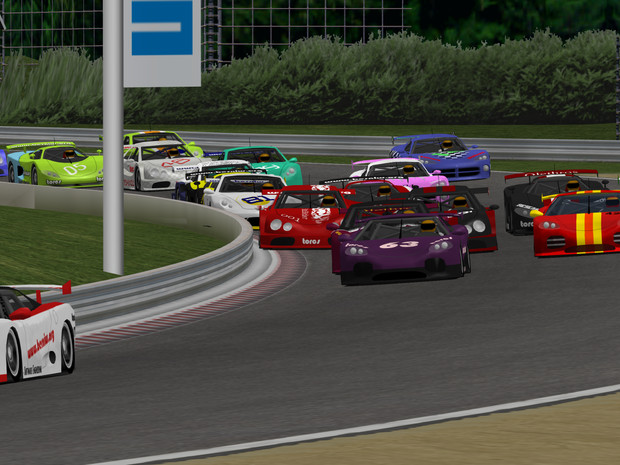
\includegraphics[height=70mm]{images/torcs.jpg}\\[1cm]

%----------------------------------------------------------------------------------------
%       DATE SECTION
%----------------------------------------------------------------------------------------

{\large \today}\\[3mm] % Date, change the \today to a set date if you want to be precise
{\large Version \docversion}\\[1.5cm]

%----------------------------------------------------------------------------------------
%       LOGO SECTION
%----------------------------------------------------------------------------------------


\includegraphics[height=13mm]{../images/logo.png} % Include a department/university logo - this will require the graphicx package

%----------------------------------------------------------------------------------------

% \vfill % Fill the rest of the page with whitespace

\end{titlepage}

  \end{titlepage}

  
  \clearpage

  \tableofcontents
  \addcontentsline{toc}{section}{Table de matière}
  
  %\vfill
  %\begin{center}
  %  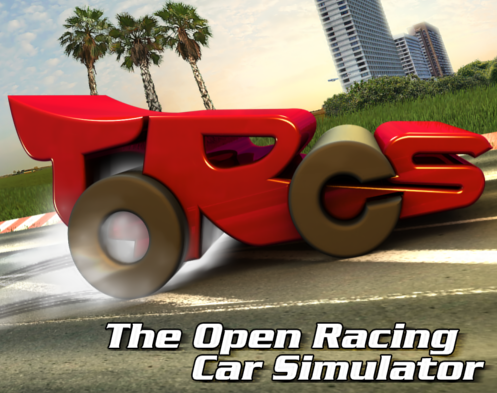
\includegraphics[height=90mm]{images/torcs.png} 
  %\end{center}

  \clearpage
  
  \renewcommand{\labelitemi}{$\bullet$}
  \renewcommand{\labelitemii}{$\circ$}
  \renewcommand{\labelitemiii}{$\diamond$}
  \renewcommand{\labelitemiv}{$\ast$}
  
  \section{Rappel des objectifs}

	Nous devrons développer une bibliothèque indépendante du domaine dans lequel l'agent évolue. 
	Elle fournira plusieurs algorithmes de base de l'apprentissage par renforcement  (Q-Learning, SARSA, …), 
	plusieurs critères de performance, ainsi qu'une ouverture sur l'apprentissage semi-supervisé : 
	c'est à dire avec les retours de l'expert pris en compte. 
	
	Dans un premier temps, l'expert pourra simplement compenser la fonction de récompense en précisant si 
	l'agent a bien ou mal agit. Dans un second temps, si le temps le permet, l'expert pourra également agir 
	sur le choix de l'action à entreprendre lors de l'exploration de l'agent, ou encore dire à l'agent s'il 
	est temps d'exploiter ou d'explorer.
	
	Parallèlement au développement de la bibliothèque, afin d'avoir une application pratique de la théorie,
	on utilisera ces algorithmes dans le simulateur TORCS sur l'apprentissage automatique de la conduite de 
	voiture sur circuit. Nous modifierons également l'interface TORCS pour intégrer les retours positifs ou 
	négatif de l'expert, voire des retours plus complexes cités précédemment \cite{CdC}.
 
 
 \section{Choix d’implémentation}
 
 \subsection{Séparation Library/Driver}
  Permettre l'indépendance total entre les 2 entitiés : aucun fichier de la library ne peut inclure un fichier du driver.
  
  \subsection{DAction \& ActionTemplate} Permet de définir n'importe quelles actions.
  
  \subsection{QTable} Transformer un tableau à 5 dimensions en un tableau à 1 dimension pour gagner en performance.
  
  \subsection{Fonctor \& Features} Flexibilité et la généralité qu'ils apportent.
  
  \clearpage
  \section{Architecture du logiciel}

  \subsection{Architecture fichiers}
  
  Le projet est constitué de 3 dossiers principaux et 2 dossiers auxilières (documentation+rapport) :
  \begin{itemize}
   \item torcs
   \item library
   \item driver
  \end{itemize}
  
  \paragraph{torcs/}
  Ce dossier contient à son tour 3 à 4 dossiers, comme son nom l'indique il relève des fichiers TORCS :
  \subparagraph{export/} contient simplement des fichiers headers afin de communiquer avec TORCS, ils proviennent
  directement du code de TORCS et n'ont pas été modifiées.
  \subparagraph{torcs.base/} (Optionnel) Contient tous les fichiers de TORCS intacts.
  \subparagraph{torcs.torcs-1.3.4/} (Optionnel) Contient tous les fichiers de TORCS compilés.
  \subparagraph{xml/} Contient des fichiers de configuration interessants de TORCS qui seront copier
  dans le répertoire \char`\~/.torcs/ de l'utilisateur. Ils permettent entre autres de gérer la taille de 
  l'écran, mais surtout de définir des courses pour l'apprentissage des agents.
  
  Les 3 scripts contenus dans torcs/ (getTorcs,...) sont décris dans le Manuel de l'Utilisateur \cite{MdU}

  \paragraph{library/} Contient tout les algorithmes génériques d'apprentissage par renforcement, ils sont
  totalement indépendant de TORCS.
    
    \subparagraph{lib/} Sert de destination pour la bibliothèque une fois compilée
    \subparagraph{build/} Contient les fichiers compilés
    \subparagraph{src/ include/} Contient les fichiers sources : bib étant général, et sml pour l'apprentissage par renforcement.
  
  \paragraph{driver/} Contient tout les algorithmes pour l'interfacement entre la bibliothèque et TORCS.
    \subparagraph{workingState/} Contient des données déjà apprises par les algorithmes (peuvent être
    utilisé pour ne pas réapprendre de zéro).
    \subparagraph{cmake/} Contient des fichiers de configuration de CMake, pour permettre une compilation
    plus aisé.
    \subparagraph{data/} Contient les fichiers de données nécessaire à l'installation module du robot.
  
  
  \paragraph{./makeDriver } Compile les sources de la library, puis celle des drivers, installe tout les fichiers
  du module du robot, ainsi que les données d'apprentissage.
  
  \paragraph{./clear } Nettoie les fichiers compilés et la bibliothèque générée.
  
  \subsubsection{Ajouter un robot}
  
  Pour ajouter correctement un robot, il convient de suivre ces différentes étapes :
    \begin{itemize}
      \item Implémenter un robot : choisir si on intègre des feedbacks du clavier, si oui, il doit descendre de DriverFeedback.
   Si non, il doit descendre de Driver.
      \item Associer l'instance à un index dans smile.cpp:InitFuncPt et augmenter le nombre de robots si nécessaire
      (smile.cpp:botname, smile.cpp:botdesc, smile.cpp:NBBOTS).
      \item Dire à torcs qu'un nouvel index est disponible dans ce module en modifiant le fichier data/smile.xml
      \item Ajouter une configuration de course qui utilise cet index dans torcs/xml/dtmraceX.xml.
      \item Recharger le tout avec ./makeDriver
  \end{itemize}

  
  \subsubsection{Lancer un apprentissage}
  
  Pour lancer un apprentissage, on utilisera ./learnIA <index> [<cpu>]. \\[0.4cm]
  Avant de lancer un apprentissage, vérifié que le robot a bien son paramètre learn à true, 
  sauf si vous voulez au contraire visualiser ces performances sans $\epsilon$-greedy.\\[0.4cm]
  Une fois l'apprentissage lancé, il faut également prendre en compte le paramètre ``restrictive\_learning''
  de votre robot, s'il est à true, l'affichage durant l'apprentissage sera moindre car il n'affichera
  et ne sauvegardera que les apprentissages ``pas trop mauvais''.
  
  
  \subsection{Developpement}
  Le projet a été conçu sous une architecture cmake, et pleinement fonctionnelle pour l'IDE Kdevelop (bien que cmake
  permettent d'utiliser n'importe quel IDE).
  
  \section{Description du code}
    \subsection{Eléments utilisés}
      \subsubsection{Boost}
      On utilise plusieurs fonction de Boost :
      \begin{itemize}
       \item les vectors pour ne pas réinventer la roue
       \item les unordered\_map implémenté via un hachage pour gagner en performance (au lieu d'un arbre)
       \item la serialization pour sauvegarder/restaurer les objets facilement en xml
       \item les mutex pour faire de l'exclusion mutuelle entre processus
       \item filesystem pour tester facilement l'existence d'un fichier
       \item les functors pour facilité la généralisation du code
      \end{itemize}

      \subsection{TORCS}
      On utilise directement ce simulateur dans lequel on intègre notre propre module.\\[0.4cm]
      On y utilise notament :
      \begin{itemize}
       \item car.h pour avoir les caractéristiques de la voiture
       \item track.h pour connaître celles de la route
       \item robottools.h pour faire des calculs et récupérer des capteurs locaux
       \item tgfclient.h pour récupérer les évènements claviers
      \end{itemize}

      Il convient de lire obligatoirement le tutoriel de TORCS sur les robots pour pouvoir se familiariser au developpement
      de ce projet \cite{TORCS_Tuto}.
    \subsection{Eléments produits}
      \subsubsection{Library}
      \begin{itemize}
       \item Q-Learning 
       \item Q-Learning($\lambda$) avec historique
       \item Q-Learning($\lambda$) par descente de gradient $Q(s,a) = \theta_{0} + \sum\limits_{i=1}^n \theta_{i} \times f_{i}(s,a)$
      \end{itemize}
      \begin{itemize}
       \item Sarsa
       \item Sarsa($\lambda$) avec historique
      \end{itemize}
      
      Chacun avec la possibilité de choisir si la trace est accumulative ou non (s'ils ont une trace).
      
      \begin{itemize}
       \item Actions/Etats discrétisés/continues génériques
       \item Fonctions d'approximation par tiling prédéfini
      \end{itemize}

      
      \subsubsection{Driver}
      
      \paragraph{Liste robots prédéfinis et interfacé avec torcs}

      \begin{center}
      \begin{scriptsize}
	\begin{tabular}{|c||c|c|c|c|c|c|}
	  \hline
	  Index & Algorithme & Etat & Action & Feedback & Classe \\ \hline \hline
	  0 & Q-Learning & distance au centre,  & direction & Sans & QLearnDiscr \\ 
	  & & tangente à la route & & & \\ \hline
	  
	  1 & Q-Learning($\lambda$) & distance au centre, & 
	      direction,  & Sans & QLearnDiscr2 \\ 
	      & & tangente à la route & 4 actions vitesse & & \\ \hline

	    2 & Q-Learning($\lambda$)  & distance au centre, &
	      direction, & Sans & QLearnGen \\ 
	  & par descente de gradient & tangente à la route & 4 actions vitesse & & \\ \hline

	    3 & Q-Learning($\lambda$)  & distance au centre, &
	      direction, & Contrôle & QLearnGenCmplx \\ 
	      & par descente de gradient & tangente à la route & 4 actions vitesse & & \\
	      &  & vitesse &  & & \\
	  &  & prochain virage &  & & \\ \hline
	  
	    4 & Q-Learning($\lambda$)  & distance au centre, &
	      direction, & Superviseur & QLearnGenFdb \\ 
	      & par descente de gradient & tangente à la route & 4 actions vitesse & & \\  \hline
	  
	    5 & Sarsa($\lambda$)  & distance au centre, &
	      direction, & Contrôle & SarsaFdb \\ 
	      & & tangente à la route, & & & \\ 
	      & & vitesse & & & \\  \hline

	\end{tabular}
      \end{scriptsize}
      \end{center}
      
      \begin{itemize}
       \item TWorld défini des fonctions de récompenses, de discrétisation, ... tout ce qui a un rapport avec le monde de TORCS
       \item TFeature prédéfini des fonctors pour les approximations de fonction dans le monde de TORCS
       \item Driver fourni les méthodes de bases d'intégration d'un agent conducteur
       \item DriverFeedback fourni les méthodes nécessaires à la récupération des évènements claviers
      \end{itemize}
      
      La fonction de récompense fonctionne de cette manière :
	  le conducteur est récompensé en fonction de la vitesse s'il reste sur les limites de la route

    \subsection{Paramètres d’implémentation}
    
    \subsubsection{À la compilation}
    Durant la compilation de TORCS, on peut choisir ou non la version debug (retirer --enable-debug dans 
    buildTorcs).\\[0.4cm]
    
    Durant la compilation du projet, on peut choisir la version release ou debug, modifier la première
    ligne de makeDriver et les options du CMakeLists.txt.

    \subsubsection{Dans le code}
  
     Il y a de nombreux paramètres défini pour un robot, en particulier on pourra trouver :
     \begin{itemize}
      \item la structure LearnConfig qui définit si l'apprentissage est restrictif (non enregistré si les 
	  performance sont trop mauvaise)
      \item learn : défini si l'agent apprend ou non
      \item DECISION\_EACH : fréquence de décision d'un agent
      \item ACTIONS\_DIRECTION : le nombre d'actions possibles pour diriger la voiture
      \item lambda : l'importance de l'historique durant l'apprentissage
      \item lrate : le taux d'apprentissage
      \item discount : l'importance du prochain état durant l'apprentissage
      \item epsilon : politique $\epsilon$-greedy
      \item road\_width : la largeur considérée pour la route
      \item total\_angle : l'angle total considéré
      \item total\_speed : la vitesse total considérée
      \item aux 3 derniers paramètres il faut associer un nombre d'entier pour les discrétiser
      \item simu\_time : le temps de simulation pour une course
      \item le choix des associations de dimension pour les fonctions d'approximation
      \item les malus pour sortie de route dans la fonction de récompense
     \end{itemize}

     
     
     
     
\addcontentsline{toc}{section}{Références}
\bibliographystyle{../dependance/apalike}
\bibliography{../dependance/biblio}

\end{document}



